\def\b0{{\bf 0}}
\def\ba{{\bf a}}
\def\bb{{\bf b}}
\def\bc{{\bf c}}
\def\bd{{\bf d}}
\def\be{{\bf e}}
\def\bg{{\bf g}}
\def\bh{{\bf h}}
\def\bi{{\bf i}}
\def\bj{{\bf j}}
\def\bk{{\bf k}}
\def\bl{{\bf l}}
\def\bm{{\bf m}}
\def\bn{{\bf n}}
\def\bo{{\bf o}}
\def\bp{{\bf p}}
\def\bq{{\bf q}}
\def\br{{\bf r}}
\def\bs{{\bf s}}
\def\bt{{\bf t}}
\def\bu{{\bf u}}
\def\bv{{\bf v}}
\def\bw{{\bf w}}
\def\bx{{\bf x}}
\def\by{{\bf y}}
\def\bz{{\bf z}}


\def\bSigma{{\bf \Sigma}}
\def\bA{{\bf A}}
\def\bB{{\bf B}}
\def\bC{{\bf C}}
\def\bD{{\bf D}}
\def\bE{{\bf E}}
\def\bF{{\bf F}}
\def\bG{{\bf G}}
\def\bH{{\bf H}}
\def\bI{{\bf I}}
\def\bJ{{\bf J}}
\def\bK{{\bf K}}
\def\bL{{\bf L}}
\def\bM{{\bf M}}
\def\bN{{\bf N}}
\def\bO{{\bf O}}
\def\bP{{\bf P}}
\def\bQ{{\bf Q}}
\def\bR{{\bf R}}
\def\bS{{\bf S}}
\def\bT{{\bf T}}
\def\bU{{\bf U}}
\def\bV{{\bf V}}
\def\bW{{\bf W}}
\def\bX{{\bf X}}
\def\bY{{\bf Y}}
\def\bZ{{\bf Z}}


%package list
\documentclass[conference]{IEEEtran}
\IEEEoverridecommandlockouts
\let\labelindent\relax
% \usepackage{breqn}
\usepackage{enumitem}
\usepackage{fleqn}
\usepackage{cite}
\usepackage{graphicx}
\usepackage[varg]{newtxmath}
\graphicspath{ {images/} }
\usepackage{pdfpages}
\usepackage{wrapfig}
\usepackage{fancyhdr}
\usepackage{lastpage}
\usepackage{lettrine}
\usepackage{amsmath}
% \usepackage{titlesec}
\usepackage[colorinlistoftodos]{todonotes}
\usepackage{float}
\usepackage[font={footnotesize}]{caption}
\usepackage[numbers,sort,square,compress]{natbib}
\usepackage[para]{footmisc}
\usepackage{xcolor}
\setlength{\belowcaptionskip}{-12pt}
\newcommand{\highlight}[1]{%
  \colorbox{red!50}{$\displaystyle#1$}}

% \usepackage{parskip}
% \setlength{\parskip}{0.02\baselineskip}

% \fancypagestyle{plain}{
%   \fancyhf{} % sets both header and footer to nothing
% \renewcommand{\headrulewidth}{0pt}
%   \fancyhead[C]{2018 International Conference on Indoor Positioning and Indoor Navigation (IPIN), 24-27 September 2018, Nantes, France}% Right header

% }
\pagestyle{plain}% Set page style to plain.

% \pagestyle{fancyplain}
% \fancyhf{}
% \renewcommand{\headrulewidth}{0pt}
% \fancyhead[C]{2018 International Conference on Indoor Positioning and Indoor Navigation (IPIN), 24-27 September 2018, Nantes, France}
\DeclareMathOperator*{\argmin}{argmin}
% \usepackage{titlesec}

% \titlespacing*{\section}{0pt}{1pt plus 2p}{1ex}
% \titleformat*{\section}{\fontsize{12}{12}\bfseries}
% \titleformat{\section}
%        {\normalfont\fontfamily{phv}\fontsize{12}{17}\bfseries}{\thesection}{1em}{}

% \titleformat{\subsection}
%        {\normalfont\fontfamily{phv}\fontsize{12}{17}\bfseries\itshape}{\thesubsection}{1em}{}

\begin{document}
%Here goes the title

\title{Scalar Feedback based Joint Time-Frequency Precoder
  interpolation for  MIMO-OFDM Systems}


%Authors List

 \author{\authorblockN{Author 1, Author 2, Author 3}
 \
 \authorblockA{Department of Electrical Engineering, Indian Institute of Technology Bombay}
% \thanks{Parts of this work was supported by the Bharti Centre for Communication in
% IIT Bombay, and the Visvesvaraya
% PhD Scheme of Ministry of Electronics \& Information Technology,
% Government of India (implemented by the Digital India Corporation).
% }}
}
\maketitle

\thispagestyle{plain}
%Main body starts



% \noindent We consider problem of quantization and interpolation of
% time and frequency varying precoding matrices in wireless MIMO
\begin{abstract}
In a limited feedback MIMO channel, the performance of the channel can improve significantly if the transmitter knows the channel state information(CSI). The receiver knows the channel information, and it feeds back to the transmitter. However, it is not possible to feedback complete information for a limited-feedback OFDM channel since the channel information for multiple subcarriers consumes a large amount of data. Therefore to resolve this problem, the orthonormality structure of the precoder matrix is exploited to make its one-to-one mapping to a minimal number of scalar parameters. The Precoder matrix is decomposed using Givens Rotation. For an i.i.d. flat-fading Rayleigh channel, these parameters are independent, which makes its quantization and interpolation easy. We propose an efficient method for quantization of the channel state information at the receiver by using adaptive delta modulation for successive time interval. We also propose a method for joint time-frequency interpolation of the channel information at the transmitter. 153-words
\end{abstract}

\section{Introduction}
\label{intro}
% no need to write the numbers in your introduction. You start by explaining what is happening currently and then propose your solution.

The use of multiple antennas at the transmitter and receiver can significantly enhance the performance of wireless systems. Moreover, in these multiple-input multiple-output (MIMO) wireless systems, the transmitter can perform better resource allocation if channel state information (CSI) is made available at the transmitter, both to improve data rates and reduce BER~\cite{love2008overview}. To this end, feeding back the CSI from the receiver to the transmitter efficiently is necessary. In wireless systems that use orthogonal frequency division multiplexing (OFDM), the feedback needs to be provided to the transmitter across all subcarriers, and this places a large feedback demand. However, since the CSI varies gradually in both time and frequency, effective techniques to reduce feedback overheads exist, using frequency domain interpolation temporal prediction. In particular, knowledge of the precoding matrices (that are typically the orthonormal right singular vectors of the channel matrix) is essential to achieve link capacity, as well as to parallelize the channel. In this paper, we focus on the problem of tracking the precoders of a MIMO-OFDM system across time and frequency for efficient CSI feedback.

The problem of effective quantization and feedback of precoders for MIMO-OFDM has attracted significant attention in recent years. Many approaches involve codebook design over the Grassmann manifold~\cite{mondal2007quantization,schwarz2013adaptive,5946308} or the Stiefel Manifold \cite{6891198,Gupt1905:Predictive}, wherein the manifold structure of the precoders is used to obtain tangents for predictive quantization and interpolation across time and frequency. While these methods have been shown to be very effective for precoder feedback,  they involve operations over higher dimensional manifolds. In particular, optimization and interpolation is complicated, especially for manifolds where geodesic paths for interpolation may be difficult to obtain, especially for joint time-frequency predictive coding. An alternate approach is to parametrize the precoding matrices using scalar parameters. The space of unitary matrices parameterized into independent scalar parameters that correspond to Givens rotations and Household Transformations of the unitary precoding matrices \cite{4114278,4556174}. These approaches have been combined with adaptive delta modulation effectively track precoding matrices both in the time~\cite{4114278} and frequency domains~\cite{4556174}, albeit separately.

In this paper, we propose a method for exploiting the joint time-frequency correlation of the precoder's scalar parameters on the transmitter using CSI feedback. Typical approaches to predictive quantization and interpolation do not exploit the joint time-frequency correlation to enhance the precoder estimate at the transmitter. However, exploiting the correlations jointly not only reduces the feedback requirement, it also is able to enhance the precoder reconstruction accuracy. Further, the independence of the scalar parameters reduces the problem to interpolation of separate scalar valued function, as opposed to operations over tangent spaces in manifolds~\cite{Gupt1905:Predictive}. Simulations reveal that the proposed method offers matches the performance of manifold based approaches with a much lower implementation complexity and fewer number of bits.


The rest of this paper is organized as follows: Section~\ref{section2} described the system model and the precoder feedback and interpolation techniques. Section~\ref{section3} compares the BER and achievable rates for our proposed methods with that of past work. Finally, Section~\ref{section4} concludes with discussions on future work.

%Since $H=U\Sigma V$, it is sufficient to quantize V*(precoder) and send this information back. In an OFDM channel, this data consumes significant amount of bits and therefore, sending the complete data could consume too much bandwidth data. For e.g. an OFDM channel with 4 transmitters, 2 receiver antennas, and 64 subcarriers would require 64*(no. of bits required to send one precoder ~ 12-16 bits) ~ 896 bits per frame. This information could be significantly reduced if we provide better quantization and interpolation techniques/strategies. Also, the matrices which need to be fed back could be broken down into independent scalar parameters. These scalar quantities could be later quantized and interpolated.

In this paper, we propose a method for predictive quantization in the time domain over the subcarriers of a MIMO-OFDM system using scalar parameters. We also exploit the joint time-frequency correlation of these scalar parameters on the transmitter side. TODO how we solve it?

The rest of this paper is organized as follows: Section~\ref{section2}, we start by explaining the system model and the method for scalar quantization \& interpolation of the precoder matrix. In \ref{section3}, we perform various simulations for our approach and show the benefits from the improved BER rates and Achievable Rate.
%Since $H=U\Sigma V$, it is sufficient to quantize V*(precoder) and send this information back. In an OFDM channel, this data consume significant amount of bits and therefore, sending the complete data could consume too much bandwidth data. For e.g. an OFDM channel with 4 transmitters, 2 receiver antennas, and 64 subcarriers would require 64*(no. of bits required to send one precoder ~ 12-16 bits) ~ 896 bits per frame. This information could be significantly reduced if we provide better quantization and interpolation techniques/strategies. Also, the matrices which need to be fed back could be broken down into independent scalar parameters. These scalar quantities could be later quantized and interpolated.
% Broad summary of your work, come to your problem definition.



\section{System Model}
For a MIMO-OFDM system with $N_T$ transmitter and $N_R$ receiver
antennas, each subcarrier $i$ with time instant $t$ could be modelled as a flat-fading MIMO channel. This flat-fading MIMO channel can be modelled as
\label{section2}
\begin{equation}
\by_{i,t} = \bH_{i,t} \bx_{i,t}+ \bf{\eta_{i,t}}
\end{equation}
where the channel matrix is
$\bH_{i,t} \in \mathbb{C}^{N_R \times N_T}$; the input is
$\bx_{i,t} \in \mathbb{C}^{N_T}$; the output is
$\by_{i,t} \in \mathbb{C}^{N_R}$ and the complex additive white
Gaussian noise is $\eta$ whose distribution is
${\mathcal{CN}}(0,I_{N_R})$. We consider the case where $N_R <
N_T$. The thin SVD of $\bH$ is given by
$\bH_{i,t} = \bU_{i,t} \Sigma_{i,t} \bV_{i,t}^{H}$, where
$\bU_{i,t} \in \mathbb{C}^{N_R \times N_R}$,
$\Sigma_{i,t} \in \mathbb{C}^{N_R \times N_R}$ and
$\bV_{i,t} \in \mathbb{C}^{N_T \times N_R}$. $\bU_{i,t}$ and
$\bV_{i,t}$ are matrices whose columns are orthonormal, and
$\Sigma_{i,t}$ contains the singular values
$\sigma_1 \geq \ldots \geq \sigma_{N_T} > 0$ of $\bH_{i,t}$. The
entries of $\bH_{i,t}$ are assumed to be distributed
i.i.d. $\tilde{\mathcal{N}}(0,1)$. To obtain a precoder at the
transmitter, we need to quantize and feed back information about
$\bV_{i,t}$ for each subcarrier.


% Givens rotation definition and how we are decomposing, Theta- pdf = 2lsin(theta)(2l-1).\cos(theta) 0 $\leq$ Theta $\leq$ pi/2.
% Householders' transformation and how we are decomposing. -pi$\leq$ phi $\leq$ pi. Uniformly distributed.
% Low-complexity quantization scheme based on a further parameterization of a vector in
% terms of a minimal number of independent scalar parameters. In particular, we consider its application to CSI feedback in slowly time-varying MIMO channels


\subsection{Scalar Parametrization}
\label{givens}
The degrees of freedom in the $\bV_{i,t}$ matrices is smaller than the
number of real entries in the matrix because of the geometrical
structure between the columns of the matrix~\cite{4114278}. The
orthonormal matrix $\bV_{i,t}$ with $N_T$ rows and $N_R$ columns can be
decomposed as TODO
\begin{equation}
\textbf{V} = \Bigg[\prod_{k=1}^{N_{R}} \bD_{k} \big( \phi_{k,k},\ldots , \phi_{k,N_{R}} \big) \: \Bigg\{ \prod_{l=1}^{l=N_{T}-k} \bG_{N_{T}-l,N_{T} -l+1} \big( \theta_{k,l}\big) \Bigg\} \Bigg] \: \tilde{\bI}
\end{equation}
where $D_{k}$ is the diagonal matrix given as $D_{k}\big(\phi_{k,k},
\ldots, \phi_{k,N_T } \big)$ =  $\mbox{diag}\big( {\bf 1}_{k-1},
e^{j\phi_{k,k}},\ldots, e^{j\phi_{k,N_T }}  \big)$, ${\bf 1}_{k-1}$ is
represents  $k-1$ ones, and the $N_R \times N_T$ matrix $\tilde{\bI}$
= $\big[\bI_{N_R }, {\bf 0}_{N_T ,N_T -N_R }\big]^{T}$, and
\begin{equation}
G_{m-1,m}\big(\theta\big)  =
\begin{bmatrix}
I_{m-2} & & & \\
& \cos\theta & -\sin\theta & \\
& \sin\theta & \cos\theta & \\
& & & I_{t-m}
\end{bmatrix}
\end{equation}
Thus, for a $4 \times 2$ orthogonal matrix $\bV_{i,t}$, we have
\begin{align*}
  \bV_{i,t} & =
  \bD_{1}(\phi_{1,1},\ldots,\phi_{1,4})\bG_{3,4}(\theta_{1,1})
  \bG_{2,3}(\theta_{1,2}) \bG_{1,2}(\theta_{1,3})\times\\
& \bD_{2}(\phi_{2,2},\phi_{2,3},\phi_{2,4}) \bG_{3,4}(\theta_{2,1}) \bG_{2,3}(\theta_{2,2})\tilde{\bI}
\end{align*}
Here, $\phi_{k}$s are referred to as phases; their collection is given by $\Phi and $$\theta_{l}$s as rotation angles; their collection is given by $\Theta$. $\phi_k \in (-\pi, + \pi]$ is uniformly distributed
between the two extremes\cite{4114278}, while $\theta_l$
is distributed as
\begin{equation}
p(\theta) = 2l(\sin\theta)^{2l-1}\cos\theta, \theta \in \left[0, \frac{\pi}{2}\right) \mbox{ for } l = 1,2,\ldots,N_T -1
\end{equation}
The $\phi_k$ and $\theta_l$ are statistically independent, making this
representation useful for tracking them separately across time, as
explained in the following subsection. The total number of parameters
obtained from the decomposition of a complex orthogonal matrix
$N_{T} \times N_{R} $ is $N_{R}(2N_{T} - N_{R})$~\cite{4114278}. The
number of $\phi_i$ parameters is $N_{R}(2N_{T} - N_{R}-1)/2$ while the
number of $\theta$ parameters is $N_{T}(2N_{T} - N_{R}+1)/2$.
\begin{figure}
\includegraphics[width=0.5\textwidth]{images/new-adpm.pdf}
\caption{\label{fig:adpm-fig}Subcarriers which need to be quantized}
\label{ber_overvie}
\vspace{-5pt}
\end{figure}
% To exploit the interpolation of time \& frequency jointly at the transmitter, feedback bits are sent in an alternating fashion as shown in the figure.

\subsection{Differential Quantization - Channel Tracking}
\label{quantiz}
For a channel that varies slowly with time, ADPM is an effective
method for tracking parameters over time using very few bits (often
just one bit). For example, while tracking a process $x_n$, at time
$n$, the one-bit jump $\beta_{n} = Q(x_{n} - \hat{x}_{n-1})$, where
$x_n$ is the unquantized value and $\hat{x}_{n-1}$ is the unquantized
(accurate) value, the quantization function $Q(x)$ is given as
\begin{equation}
  Q(x)=\begin{cases}
    1, & \text{if $x>0$}.\\
    -1, & \text{otherwise}.
  \end{cases}
\end{equation}
Thus, the quantied vector $\hat{x}_n$ evolves with time as
\begin{equation}
\hat{x}_{n} = \hat{x}_{n-1} + \beta_{n}\Delta_{n} \mbox{ where }
\label{delta_eqn}
\Delta_{n} = \begin{cases}
    M \Delta_{n-1}, & \text{if $\beta_{n} = \beta_{n-1}$}\\
    \Delta_{n-1}/m , & \text{if $\beta_{n} \neq \beta_{n-1}$}.
  \end{cases}
\end{equation}
Here we initialize delta using $\Delta_1 = |x_{2}-\hat{x}_1|$.

To quantize the subcarriers efficiently and exploit the joint
time-frequency interpolation at the transmitter, we select the
subcarriers for quantization in an alternating fashion as shown in
Fig.~\ref{fig:adpm-fig}. The figure shows the channel evolution of an
$N$ subcarrier MIMO-OFDM system with the subcarriers that are
quantized. Every $p$-th subcarrier starting with $0$ is quantized for
even time instances, where, $p$ is the gap between two quantized
subcarrier indices. For odd time instances, subcarriers at the
position $pk+q$ for $k = 0,1,..., \frac{N-1}{p}$ with $q =
{\frac{p}{2}}$.

For the adaptive channel tracking scheme, the arrows in
Fig.~\ref{fig:adpm-fig} show how previous quantized values along with
the 1-bit enhancement are used to find the new quantized value. Since
we use a single bit adaptation, the amount of feedback required is 1
bit for each scalar parameter that is being tracked. On an average,
this can be reduced by half if we transmit only $\Theta$ values for
one-time instance and only $\Phi$ values for the next time instant in
an alternating fashion (the untransmitted value is assumed to be the
same as that at the previous instant). In this case, the average
number of bits required to quantize a channel matrix will be
$N_{T}(2N_{T} - N_{R})/2$.

One issue that is associated with the tracking the $\phi_i$ parameters
is that they may change abruptly (cite the figure) between $-\pi$ and
$\pi$ due to jumps of $2\pi$. We have avoided this by unwrapping the
phases to facilitate continuous tracking.
\subsection{Joint Time Frequency Interpolation}
\label{interp}
After obtaining the $\beta$ values (using the single bit feedback) at
the transmitter, we can construct the precoder at subcarrier indices
$pk$ or $pk+q$. To construct the rest of the subcarriers, we will use
precoder parameters from both the past and future and time instances
to do the interpolation (using backtracking to ensure causality). In
Fig.~\ref{fig:adpm-fig}, each parameter is interpolated using the
neighbouring subcarriers using bilinear interpolation (equivalent to
linear interpolation in two dimensions). These interpolated values and
then used to reconstruct the precoding matrices all together. Thus,
the approach here is able to exploit the time and frequency
correlation jointly to enhance performance.

One reason why a linear predictive quantization is preferred is
because the underlying parameters can generally be thought to emerge
from an autoregressive (AR) process. For such processes, it is well known
that linear prediction based on past samples is optimal. Even though
the $\Theta$ and $\Phi$ parameters do not manifest as AR processes,
for small changes, a linear approximation works sufficiently
well, as in the description in~\cite{4114278}, although that was
limited to tracking the temporal evolution of the parameters.

\section{Simulation and discussion}
\label{section3}
We present some simulations of the scalar feedback based joint
time-frequency predictive quantization outlined in the previous section. performed simulations to analyse the performance of the proposed quantization and interpolation method for slowly time-varying MIMO OFDM channel. Channel is simulated using the typical Jakes Model for both ITU Vehicular-A channel and ITU Pedestrian Channel. Performance is measured by averaging over 10 channel realizations with 100 simulations each. The normalised doppler frequency $f_{norm} = f_{max}.T_s$ is set to $3.5\times10^{-4}$ with symbol time period $T_d = 5\times10^{-8} s$. For both vehicular and pedestrian channel, $N_T=4$ and $N_R=2$. Therefore, the total number of parameters are $N_{R}(2N_{T} - N_{R}) = 12$ with 5$\theta$’s and 7$\phi$’s. There are 1024 subcarriers in Vehicular channel and 64 subcarriers in the Pedestrian Channel. We take s = 33/9 for Vehicular and pedestrian channel respectively I.e. 32/8 equally spaced subcarriers with indices 33t/9t, t = 0,1, … , 31 and 0,1, .. ,7 respectively.

\subsection{Initial Quantization}
For the first and the second simulations/time instances we use of $\textbf{B}$ = 10 bits for quantizing each parameter for effective quantization/initialization. Therefore, the number of bits for each subcarrier = $10\times12$ = 120. Quantization is performed as given in Section~\ref{section2}.

Simulation: BER is calculated by averaging over all the simulations. For Vehicular Channel, 1024 subcarriers are used with doppler frequency – and sampling rate = $10^{5}$

Initialization is performed by using $10\times12$ bits for each subcarrier for the initial two time frames. Later, the quantization will take place in the time-domain using one bit for each parameter. Since the bit budget is low and we are considering slowly varying channels, therefore, either theta or phi parameters are sent alternatingly in the time domain while keeping the unsent parameters equal to their previous values as show in the Figure \ref{adpm-fig}. Here $\Theta$ is the the collection of all $\theta$'s and $\Phi$ is the collection of all $phi$'s. This brings down the bit budget to average of 5(Size of $\Theta$) and 7(Size of $\Phi$) i.e. 6 bits average per fed back subcarrier.

{ADPM Design}: The decrement/decay rate is given by $\bm$ and increment/growth rate is given by $\bM$ in the Equation~\ref{delta_eqn} . The ratio of $m/M$ is fixed at 2.5 i.e. higher decay than increment of the delta values. This way, quantized values are able to follow the curve more precisely. Also, need to describe the initialization of the Delta values required in the quantization process. Need to cite that paper.

Performance Measurements:
Since the Precoding matrices fundamentally lie on the Stiefel manifold, therefore, we are using the chordal distance parameter to measure the effectiveness of the quantization method used by us. Later we are comparing the BER rates with the ideal completely fed back subcarriers.

Using the idea of joint interpolation given in the other paper.

%talk about this in the simulations, that would be more relevant
Since $\Delta_{n} = M\Delta_{n-1} or \Delta_{n-1}/m $, we found empirically that $m=2.4*M$ i.e. decay

\begin{figure}
\includegraphics[width=0.5\textwidth]{images/pedestrian.pdf}
\caption{BER vs SNR for pedestrian channel}
\label{ber_overview}
\vspace{-5pt}
\end{figure}

\subsection{Performance Measurement}

\label{setting}



\noindent Since the Precoding matrices fundamentally lie on the Stiefel manifold, therefore, we are using the chordal distance parameter to measure the effectiveness of the quantization method used. Later we are comparing the BER rates with the completely fed back subcarriers. Or simulations and discussions part 2 criteria could be used. Done similar work as in \cite{4114278} but along with that we have joint interpolated in time and frequency at the transmitter using the fundamental scalar parameters obtained. To lower the number of bits we have used the method of interpolation and have achieved significant improvement over predictive quantization method in \cite{6891198} and also in \cite{Gupt1905:Predictive} which tried to use joint interpolation over the tangent space in the Stiefel Manifold. In fact, we use joint interpolation of the scalar parameters which are easy to use and give better quantization than any of the above methods.

The advantage they had over the number of bits due to the 6 bit codebook in \cite{6891198,Gupt1905:Predictive} is also achieved by us by using smart interpolation techniques, i.e. by dropping the feedback bits in alternating time instances as it is still going to follow the scalar parameters without much difference.

The problem of values hopping between $\pi$ and $-\pi$ is also tackled by wrapping the values around which we can show works nicely. The only drawback is that while initializing the parameter, they go out of their actual range and therefore using a uniform quantizer over the prescribed range does not work. But since most of the values lie between the given range we can use most of the initialization bits quantizing the parameters uniformly between the [-$\pi$ , $\pi$] and using smaller amount of bits between the range outside that which could go up to $-3\pi$ and $3\pi$, i.e. we are covering 300% more range outside the given area and that works mostly fine for the rest of the values.

Using the idea of joint interpolation given in the other paper.

\begin{figure}
\includegraphics[width=0.5\textwidth]{images/vehicular_ber.pdf}
\caption{BER vehicular plot comparison between our method and \cite{Gupt1905:Predictive}}
\label{ber_overview}
\vspace{-5pt}
\end{figure}
%Qtisn error with 1000 chan evols
%Qtisn error with 100 chan evols
%BER
%Achievable rat
\section{Conclusions and Future Work}
\label{section4}

We could reduce more by seeing the effect of sigma values (power distribution). We can save the bits by not sending for those which have very low sigma values. This could result in a very robust method.

\vspace{-4pt}



% \section{Acknowledgment}

% % \label {section6}

% % \input{sections/6_section.tex}

% Parts of this work was supported by the Bharti Centre for Communication in

% IIT Bombay, and the Visvesvaraya

% PhD Scheme of Ministry of Electronics \& Information Technology,

% Government of India, being implemented by Digital India Corporation.





\renewcommand{\bibfont}{\footnotesize}

\bibliography{IEEEabrv,main}

\bibliographystyle{IEEEtran}

\end{document}
